% diagram_clip.tex
% Visual explanation of the clip(.) operator used in the additive rule design
% (Eq. \ref{eq:additive_rule}). Designed to be \input{} from paper_wea2026.tex.
%
% Requires: \usepackage{tikz}
%
% Idea: e_prog and e_div are integer effects on a discrete label axis.
% Their sum may fall outside the available label range; clip(.) snaps it back
% to the nearest extreme label so that the additive design always yields a
% valid output linguistic term.
%
% Example shown: 3-label case, support {-1, 0, +1} mapped to {L, M, H}.
% e_prog = +1 (toward H), e_div = +1 (toward H), sum = +2 -> clipped to +1 = H.
%
\begin{figure}[h]
\centering
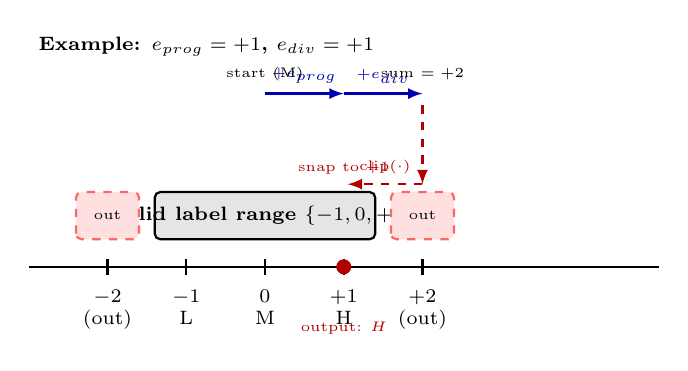
\begin{tikzpicture}[
    >=latex, font=\scriptsize,
    label/.style={font=\scriptsize\bfseries},
    tick/.style={thick},
    eff/.style={->, thick},
    clipline/.style={->, thick, dashed},
    valid/.style={fill=black!10, draw=black, thick, rounded corners=2pt},
    outside/.style={fill=red!12, draw=red!60, thick, dashed, rounded corners=2pt}
]
% ---- label axis (3L) ----
\draw[tick] (-3,0) -- (5,0);
\foreach \x/\lab in {-2/{$-2$\\(out)}, -1/{$-1$\\L}, 0/{$0$\\M}, 1/{$+1$\\H}, 2/{$+2$\\(out)}} {
    \draw[tick] (\x,0.1) -- (\x,-0.1);
    \node[align=center, below=2pt] at (\x,-0.1) {\lab};
}
% valid region
\draw[valid] (-1.4,0.35) rectangle (1.4,0.95);
\node[label] at (0,0.65) {valid label range $\{-1,0,+1\}$};

% out-of-range region (left)
\draw[outside] (-2.4,0.35) rectangle (-1.6,0.95);
\node[font=\tiny] at (-2,0.65) {out};
% out-of-range region (right)
\draw[outside] (1.6,0.35) rectangle (2.4,0.95);
\node[font=\tiny] at (2,0.65) {out};

% additive composition arrows above
\node[label, anchor=west] at (-3.0,2.8) {Example: $e_{\text{prog}}=+1$, $e_{\text{div}}=+1$};
\draw[eff, blue!70!black] (0,2.2) -- (1,2.2)
    node[midway, above, font=\tiny] {$+e_{\text{prog}}$};
\draw[eff, blue!70!black] (1,2.2) -- (2,2.2)
    node[midway, above, font=\tiny] {$+e_{\text{div}}$};
\node[font=\tiny] at (0,2.45) {start (M)};
\node[font=\tiny] at (2.0,2.45) {sum $=+2$};

% drop down to axis
\draw[clipline, red!70!black] (2,2.05) -- (2,1.05);
% clip arrow snapping back to +1
\draw[clipline, red!70!black] (2,1.05) -- (1.05,1.05)
    node[midway, above, font=\tiny] {$\mathrm{clip}(\cdot)$};
\node[font=\tiny, red!70!black] at (1,1.25) {snap to $+1$};

% final dot
\filldraw[red!70!black] (1,0) circle (2.5pt);
\node[font=\tiny, red!70!black, below=12pt] at (1,-0.15) {output: $H$};

\end{tikzpicture}
\caption{Geometric meaning of $\mathrm{clip}(\cdot)$ in Eq.~\eqref{eq:additive_rule}. The two semantic effects $e_{\text{prog}}$ and $e_{\text{div}}$ are added on the integer label axis. If their sum lies inside the valid label range it is used directly; if it falls outside (here $+2$ at three labels), $\mathrm{clip}(\cdot)$ snaps it to the nearest extreme label ($H$). The same convention applies symmetrically on the negative side and at five labels with support $\{-2,\dots,+2\}$.}
\label{fig:clip}
\end{figure}
